% Chapter 2

\externaldocument{chapter3}
\externaldocument{chapter4}
\externaldocument{chapter5}
\externaldocument{chapter1}
\externaldocument{AppendixA}
\chapter{Formalisms} % Main chapter title

\label{Chapter2} % For referencing the chapter elsewhere, use \ref{Chapter2} 


%----------------------------------------------------------------------------------------

%\section{Welcome and Thank You}
%In this chapter, acoustical characteristics of music signal that enables general MIR tasks will be introduced.We will examine the Fourier Series representations of sound waves and see how they relate to harmonics and tonal color of instruments  
To map a music to it's semantic descriptions, the signal is first transformed to a lower dimensional space. The resulting transformation is called \textit{feature}. The classifier then takes these features as input and performs the classification task. The performance of the classifier can only be as good as the information encoded in the features. In this chapter, formalisms required for the analysis of feature extraction are introduced. The raw signal is first changed to a representation that can be mathematically analysed (see Sec. \ref{rep}). This representation is then transformed to a lower dimensional space by discarding information that does not contribute to discrimination (see Sec. \ref{dimension}). The resulting reduction is then approximated to a fixed size representation (see Sec. \ref{temporal}) which is then taken as input by a multi-label classifier (see Sec. \ref{classifier}). In section \ref{training}, training procedure that can optimize feature representations for supervised classification task is discussed. 
%----------------------------------------------------------------------------------------

\section{Representation of music signal}
\label{rep}
The observed signal is traditionally represented in the time domain. The time domain is a record of what happened to a parameter of the system versus time. Standard formats use amplitude versus time. The observed signal is then discretised by sampling and stored in digital format (see \ref{sampling}). This signal in the time domain is then changed to frequency domain (see \ref{time}). This is simply because our ear-brain combination is an excellent frequency domain analyser. Currently used music signal representations for general MIR tasks are explained in section \ref{stft}.


\subsection{Sampling of continuous-time signal}
\label{sampling}
The digital formats contain the discrete version of the signal obtained by sampling continuous-time signal. Sampling is performed by measuring the value of the continuous signal every $T$ seconds. This interval $T$ is called the sampling interval or the sampling period. The sampling frequency or sampling rate ($f_{s}$) is the number of samples obtained in one second (samples per second),  
\[
 f_{s} = \frac{1}{T}.
\]
The optimum sampling rate is given by Nyquist-Shannon sampling theorem which says, the sampling frequency $f_{s}$ should be at least twice the highest frequency contained in the signal. Given the human hearing range lies between 20Hz - 20KHz, most of the digital audio formats use a standard sampling frequency of 44.4Khz. Sampling rate determines the initial dimension of the raw signal. The signal may be further down sampled if higher sampling rate does not contribute to classification performance.

\subsection{Time-Frequency transformations}
\label{time}
The digital signal is represented in the time domain with amplitude values at each time $t$. This representation has to be changed to frequency domain. Mapping from time-domain to frequency-domain is looked up on as basis transformation. 

\subsubsection{Basis transformation from time to frequency domain}
\noindent The signal in the time domain $\textbf{a}$ is a set of ordered \textit{n}-tuples of real numbers \( (a_{1},a_{2}, ...,a_{N}) \in \mathbb{R}^N \) in the vector space \textit{V}, specifically \textit{Euclidean n-space}. That is to say, a discrete-time signal can be represented as a linear combination of Cartesian basis vectors. The coefficients in linear combination are then the co-ordinates of the corresponding basis system.  
\[
\textbf{a} = (a_{1},a_{2}, ...,a_{N}) = a_{1}\textbf{e}_{1} + a_{2}\textbf{e}_{2} + ... + a_{N}\textbf{e}_{N} = \displaystyle\sum_{t=1}^{N}a_{t}\textbf{e}_{t} = \mathbb{I}\textbf{a}
\]
Where $(a_{1},a_{2}, ...,a_{N})$ are the co-ordinates of Cartesian basis formed by basis vectors $\textbf{e}_{1} ... \textbf{e}_{N}$ with $t \in \{1,2,..N\}$. The unit vector $\textbf{e}_{t} \in \mathbb{R}^{N}$ has 1 in the $t^{th}$ index and 0 everywhere else.
\bigskip

\noindent To transform to frequency domain, we need to find a set of basis vectors $\bm{\phi}_{ \omega }$ that are functions of frequencies ($\omega$). Then the co-ordinates of this basis system $c_{ \omega }$ represents the signal in frequency domain. 
\begin{equation}
\label{exp_fourier}
\textbf{a} = \displaystyle\sum_{ \omega =1}^{M}c_{ \omega }\bm{\phi}_{ \omega } = \bm{\Phi}\textbf{c} \qquad \bm{\Phi} \in \mathbb{C}^{N \times M}, \textbf{c} \in \mathbb{C}^{M}
\end{equation}
If $\bm{\Phi}$ is known, then the transformed co-ordinates $\textbf{c} = (c_{1},c_{2},..,c_{M})$ can be computed as,
\[
\textbf{c} = \bm{\Phi}^{-1}\textbf{a}
\]
$\textbf{c}$ is the transformed representation. $\bm{\Phi}^{-1}$ is the operator that transforms the signal. 

\subsubsection{Exponential Fourier Series and Fourier Transform}
From the definition of \textit{exponential Fourier Series}, any function \textit{periodic} in $\{1,2,..,T\}$ can be expanded with series of complex exponentials\cite{allen}. These complex exponentials which are functions of harmonically related frequencies($k \omega$) form basis 
\[
\bm{\phi}_{k}(t) = \frac{1}{\sqrt{T}}e^{ik \omega t} \qquad t \in \{1,2,..T\}
\] 
It is difficult to assume periodicity for a generalized signal. Hence, the Fourier series can not be applied directly and Fourier Transform was developed. By Fourier transform, quantity of each frequency component $\omega$ in an arbitrary signal $\textbf{a}(t)$ can be computed by dividing by $e^{i \omega t}$. Application of Fourier transform to a discrete signal is called \textit{Discrete Fourier Transform}
\[
c_{\omega} =  \displaystyle\sum_{t=1}^{N}a_{t}e^{-i \omega t} \qquad t \in \{1,2,...,N\}
\] 
Thus the transformation operator is,
\[
\bm{\Phi}^{-1}[ \omega ] = e^{-i \omega \textbf{t}} \qquad \textbf{t} \in \mathbb{R}^{N}, \omega \in \{1,2,..,M\}
\]
Fast Fourier Transform(FFT) is an efficient implementation of Discrete Fourier Transform(DFT) which exploits the symmetry of $sines$ and $cosines$ in the complex exponential. While DFT requires $O(N^2)$ operations, FFT requires only $O(NlogN)$ \cite{allen}. 


\subsection{STFT, Mel-Spectrogram}
\label{stft}
It is useful to perform FFT locally over short segments. This is because we are more interested in the evolution of frequency content rather than the frequency content of the entire signal. Hence, the full length signal is divided into short segments, and FFT is computed separately for each segment. This is known as \textbf{Short Time Fourier Transform (STFT)}. One common problem with STFT is the \textit{spectral leakage}, which is addressed by modifying the original signal with some window function. The most common window function is the \textbf{Hamming Window} defined as,
\begin{equation}
h[n] = 0.54 - 0.46cos(\frac{2 \pi n}{N-1})
\end{equation}
where $n \in \{1,2,..,F\}$ and $F$ is the size of window function. The signal approaches zero near $n=1$ and $n=N$, but reaches peak near $n=N/2$ \cite{specLeak}. To overcome the information loss at the ends of the window, signal is divided into segments that are partly \textit{overlapping} with each other. The distance between the start of two adjacent segments is called \textit{hop-length}. Figure \ref{fig:stftPipe} shows the extraction of spectral frames of a spectrogram. Thus, the parameters of STFT include 
\begin{itemize}
    \setlength\itemsep{0em}
    \item Choice of window function
    \item Size of each segment in $\textbf{a}$ ($F$)
    \item Hop length or stride ($s$) of the transformation operator
    \item Size of frequency dimension $M$ (also known as FFT size)
\end{itemize}

\begin{figure}[h]
       \begin{subfigure}[b]{0.6\textwidth}
        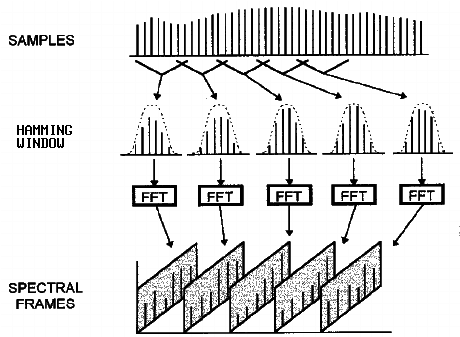
\includegraphics[width=\textwidth]{stft_pipe}
        \caption{Windowing is applied on overlapping segments\\ followed by FFT }
        \label{fig:stftPipe}
       \end{subfigure}
	    \begin{subfigure}[b]{0.4\textwidth}
        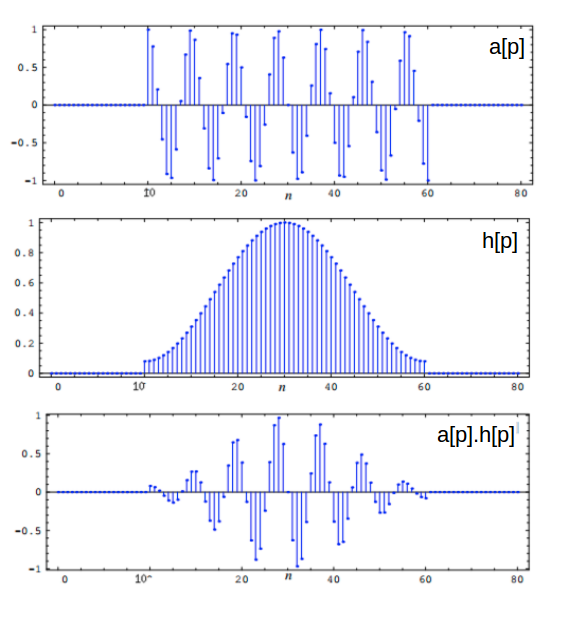
\includegraphics[width=\textwidth]{stft}
        \caption{
        Application of Hamming Window on \\a segment of input signal
        }
        \label{fig:HammingWindow}
       \end{subfigure}
       \caption{\cite{spec_dia} (a) Shows STFT Pipeline. (b) Shows the application of \\Window function}\label{fig:STFT}
\end{figure}
\FloatBarrier

\subsubsection{STFT as Convolution}
\noindent The strided operation over the signal $\textbf{a}$ is mathematically represented as a \textbf{convolution}. The resulting spectrogram has $P$ frames. The discrete STFT (\textit{slow}) for $p^{th}$ frame of signal $\textbf{a}$ is obtained as,
\begin{equation}
\label{stfteq}
\textbf{C}[p, \omega ] = \displaystyle\sum_{n=p.s}^{p.s + F}\textbf{a}[n] \Big( \textbf{h}[n-p.s] . e^{-i \omega (n-p.s)} \Big)
\end{equation}
Where:
\begin{itemize}[label=]
    \setlength\itemsep{0em}
    \item $P$: is the number of spectral frames; $p \in [1,2...,P]$ 
    \item $M$: is the dimension of discrete frequency space ; $\omega \in \mathbb{R}^{M}$
    \item $F$: is the frame length 
    \item $s$: is stride (or) hop-length to the next segment
    \item $\textbf{a} \in  \mathbb{R}^{N}$ ; $n \in [1,2,...,N]$
    \item $\textbf{h} \in  \mathbb{R}^{F}$
    \item $\omega \in  \mathbb{R}^{M}$
    \item $\textbf{C} \in \mathbb{C}^{M \times P}$
\end{itemize}
\noindent Equation \ref{stfteq} can be seen as a \textbf{discrete convolution} over the signal \textbf{a} with the operator $\textbf{W}_{STFT}$ which has finite support over the set $\{1..,F\}$ with stride $s$
\[
\textbf{C} = \textbf{a} \star \big( \textbf{h} \bm{\Phi}^{-1} \big)
\]
\begin{equation}
\label{eq:stft}
\textbf{C} = \textbf{a} \star {\textbf{W}^{(s)}}_{STFT}
\end{equation}
where $\textbf{W}_{STFT} = \textbf{h} \bm{\Phi}^{-1}$ is the STFT operator that transforms the signal $\textbf{a}$ from time to frequency domain. 
\bigskip

\subsubsection{Power spectrogram}
\noindent It is important to note that the coefficient matrix $\textbf{C}$ may be complex valued. To obtain useful metrics, we need to extract some physical quantity from the coefficients. This is where \textbf{Parseval's theorem} is used, which relates time and frequency domain components in DFT as follows \cite{allen} :
\begin{equation}
{\|\textbf{c}\|}^2 \propto {\|\textbf{a}\|}^2
\end{equation}
If \textbf{a} represents amplitude in the time-domain, then we know that the energy of a wave is related to it's amplitude as,
\begin{equation}
Energy \propto amplitude^2
\end{equation}
Thus, it can be inferred that \textbf{square} of the Fourier coefficients is proportional to the energy distributed in the corresponding frequencies. This spectrogram with squared coefficients is called the \textbf{Power Spectrum (P)}. It is often motivating to use this representation because \textit{loudness} is proportional to \textit{energy}.
\begin{equation}
\label{energy}
\textbf{P} = \textbf{C} \odot \textbf{C}
\end{equation}

\noindent The frequencies in the considered range are  grouped into bins. It is useful to do so, due to the aliasing effect of human auditory system. This is motivated by the human cochlea (an organ in the ear) which vibrates at different spots depending on the frequency of the incoming sounds.
  
\subsubsection{Mel Power Spectrogram}
\label{mel}

The \textit{mel-scale} was developed to express measured frequency in terms of psychological metrics (i.e perceived pitch). The mel-scale was developed
by experimenting with the human ears interpretation of a pitch. The pitch is linearly perceived in the frequency range 0-1000 Hz. Above
1000 Hz, the scale becomes logarithmic. There are several formulae to convert Hertz to mel. The following formula is used in this thesis\cite{speech}
\begin{equation}
\omega_{m} = 2595log_{10}\bigg(1+\frac{ \omega }{700}\bigg)
\end{equation}
where $\omega$ is the frequency in Hertz. In a mel spectrogram, the frequencies and converted to mels and then grouped into mel-spaced bins. This is done by multiplying the spectrum with \textbf{mel filter bank ($\textbf{W}_{MEL}$)}. For details about computation of mel-filter banks, refer \cite{mel}. Each filter bank is centered at a specific frequency. Hence, to compute R mel bins, we need R mel-filter banks. The resulting mel power spectrogram ($\textbf{X}$) is
\begin{equation}
\label{mel_conv}
\textbf{X} = \textbf{W}_{MEL}\textbf{P}
\end{equation}
\[
 \textbf{W}_{MEL} \in  \mathbb{R}^{R \times M}, \textbf{P} \in \mathbb{R}^{M \times P}, \textbf{X} \in \mathbb{R}^{R \times P}
\]

\noindent The above Matrix-Matrix multiplication can be represented as a convolution with window size and stride equal to $M$. We can re-write equation \ref{mel_conv} as, 
\begin{equation}
\label{mel_conv_flat}
\textbf{X}[p,\omega_{m}] = \displaystyle\sum_{k=p.M}^{p.M + K}\textbf{p}[k]\textbf{W}_{MEL}(k-p.M)
\end{equation}
Where:
\begin{itemize}[label=]
    \setlength\itemsep{0em}
    \item $\textbf{p}[k]$ = $\textbf{P}[i,j]$ ; $i = floor(\frac{k}{M})$ ; $j = k-floor(\frac{Mk}{M-1})$
    \item $\omega = k-p.M \in \mathbb{R}^{M}$
    \item $\textbf{X} \in \mathbb{R}^{M \times P}$
    \item $\textbf{p} \in \mathbb{R}^{M.P}$
    \item $\omega_{m} \in  \mathbb{R}^{R}$
\end{itemize}

\noindent Hence, we can represent mel-power spectrogram as \textbf{M-strided convolution} over \textit{flattened} $\textbf{P}$ with mel filters $\textbf{W}_{MEL}$ (i.e, the frequency axis of $\textbf{P}$ is contracted with each mel-filter) 
\begin{equation}
\label{eq:mel}
\boxed
{
  \textbf{X} = \textbf{P} \star \textbf{W}_{MEL}
}
\end{equation}  
Thus the extraction of mel-power spectrogram can be summarized in the following algorithm 
\begin{algorithm}
  \caption{$\textbf{X}$ = $R_{(MEL)}$($\textbf{a}$)}\label{alg:mel}
  \begin{algorithmic}[1]
    \Statex \textbf{Input :} $\textbf{a} \in \mathbb{R}^{N}$
    \Statex \textbf{Output :} $\textbf{X} \in \mathbb{R}^{R \times P}$
	\State $\textbf{C} = \textbf{a} \star \textbf{W}_{STFT}$
	\State $\textbf{P} = \textbf{C} \odot \textbf{C}$
	\State $\textbf{X} = \textbf{P} \star \textbf{W}_{MEL}$
  \end{algorithmic}
\end{algorithm}
\FloatBarrier

\section{Dimensionality Reduction}
\label{dimension}
The objective of dimensionality reduction is to retain only the information that contribute to discrimination and discard the rest. This is done because the \textit{representation} ($\textbf{X}$) can be large for longer audio tracks (because number of frames $P$ depends on length of the audio). In this thesis, only \textit{mel-spectrogram representation} is considered. The dimensionality reduction of input signal $\textbf{a}$ is generalized as follows,
\[
   \textbf{X} = R(\textbf{a}) \qquad R : \mathbb{R}^{N} \rightarrow \mathbb{R}^{R \times P}
\]
\begin{equation}
\label{dim_red_abstract}
   \textbf{Y} = D(\textbf{X}) \qquad D : \mathbb{R}^{R \times P} \rightarrow \mathbb{R}^{T \times W} 
\end{equation}
 
\noindent The computation of mel-spectrogram defined in the previous section can be a part of the function $R$. The dimensionality reduction is defined by function $D$. The output of reduction $\textbf{Y} \in \mathbb{R}^{T \times W}$ will be the reduced representation ($T < R$ or $W < P$). Depending on how the function $D$ is defined, the following three methods will be discussed
\begin{itemize}
  \item \textbf{Principal Component Analysis} (PCA) : Reduction by \textit{unsupervised learning}.
  \item \textbf{Mel-Frequency Cepstrum Coefficients} (MFCC) : Reduction by domain engineering.
  \item \textbf{Convolution Neural Networks} (CNN) : Reduction by \textit{supervised learning}
\end{itemize} 
\begin{figure}[h] 
\centering
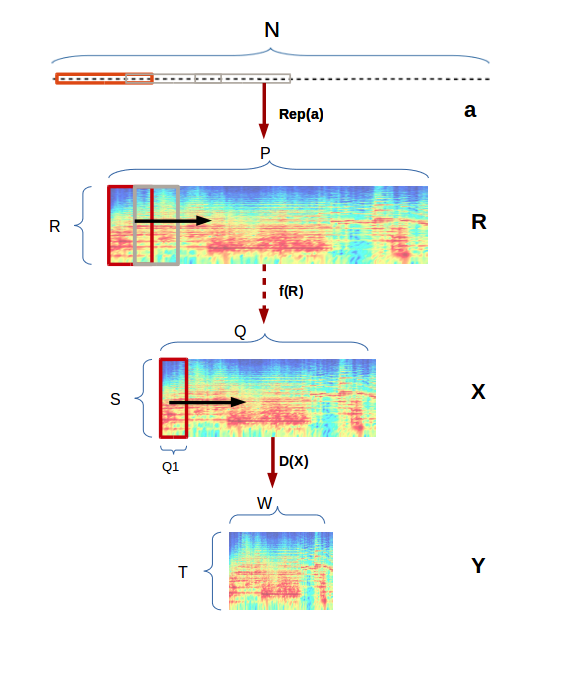
\includegraphics[width=0.7\textwidth]{dim_red}
\caption{Dimensionality Reduction Pipeline}
 \label{fig:Dimensionality Reduction}
 \end{figure}
\FloatBarrier
\bigskip

\subsection{Domain engineering Vs Unsupervised learning Vs Supervised learning}
\textit{Reduction by Domain engineering :} When the operators performing reduction are computed using the domain specific properties of the data, then the resulting reduction is said to be \textit{engineered}. Coming up with such operators is usually time-consuming and requires expert knowledge.\\
\\
\textit{Reduction by Unsupervised learning :} When the operators performing reduction are computed by exploiting the representation \textit{structure} of the data, then the resulting reductions are said to be \textit{learned} from the data. When this learning problem \textit{does not} require any labelled data, then the reduction is said to be \textit{unsupervised}.\\
\\
\textit{Reduction by Supervised learning :} When the operators performing reduction computed by exploiting the information from labelled data, then the resulting reduction is said to be obtained by \textit{supervised learning} 

\subsection{Principal Component Analysis (PCA)}
\label{pca}

The representation $\textbf{X}$ is changed to a \textit{basis} that are functions of variance between the frequency components. This is done by computing the co-variance matrix $\bm{\Sigma}$ from the data and performing \textit{orthogonal decomposition} to compute it's basis. The co-ordinates of the resulting basis system are called \textit{principal components}. The key idea for reduction is to discard the information corresponding to \textit{low variance} basis. The computation of PCA reduction operator $\textbf{W}_{PCA}$ is elaborated below,  

\begin{enumerate}[label=(\alph*)]
\item Usually, large samples (say $S$ samples) of representations from the dataset ($ \textbf{S} = [\textbf{X}_{1}, \textbf{X}_{2}, ..., \textbf{X}_{S}])$ are used to compute the co-variance matrix. The columns of $\textbf{S}$ are centred by their mean and the covariance matrix is computed as,
\[
   \bm{\Sigma} = \textbf{E}[(\textbf{S} - \textbf{E}[\textbf{S}])(\textbf{S} - \textbf{E}[\textbf{S}])^{T}] = \frac{1}{\displaystyle\sum_{s}{P_{s}}}\textbf{\^S}\textbf{\^S}^{T} \quad \in \mathbb{S}^{R \times R}
\]
The covariance matrix $\bm{\Sigma}$ is symmetric positive definite and hence belongs to space of symmetric operators $\mathbb{S}$.
\item The eigen values and eigen vectors of $\bm{\Sigma}$ are computed. At this point, we use the Orthogonal Eigenvector Decomposition Theorem and infer that eigen vectors of symmetric matrix ($\bm{\Sigma}$) form an orthogonal basis in $\mathbb{R}^{R}$. 
\[
\bm{\Sigma} = \textbf{V}\bm{\Lambda}\textbf{V}^{T} \qquad \textbf{V} \in \mathbb{O}^{R \times R}, \quad \bm{\Lambda} \in \mathbb{D}^{R \times R}
\]
The columns of matrix $\textbf{V}$ form the basis. Since the columns are orthogonal to each other, $\textbf{V}$ belongs to a space of orthogonal operators $\mathbb{O}$. $\bm{\Lambda}$ is a diagonal matrix of eigen values.

\item The eigen values represent the magnitude of variance for each frequency dimension.  Hence, eigenvectors corresponding to large eigen values gives the coordinates corresponding to greater variance. So eigen vectors corresponding to top $T$ eigen values are retained, while ignoring coordinates of lower variance. The resulting change of coordinates matrix is then $\textbf{\^V} \in \mathbb{O}^{R \times T}$
   
\item Since $\textbf{\^V}$ is orthogonal, $\textbf{\^{V}}^{-1} = \textbf{\^{V}}^{T}$, and the resulting reduction for \textit{each sample} can computed as $\textbf{Y} = \textbf{\^{V}}^{T}\textbf{X}$, where $\textbf{X} \in \mathbb{R}^{R \times P}$, $\textbf{Y} \in \mathbb{R}^{T \times P}$ and $T < R$. Thus the reduction operator is
\[
\textbf{W}_{PCA} = \textbf{\^V}^{T}
\]

\end{enumerate}   

\begin{algorithm}
  \caption{$\textbf{W}_{PCA}$ = PCA($\textbf{X}_{1}, \textbf{X}_{2},..,\textbf{X}_{S}$)}\label{alg:pca}
  \begin{algorithmic}[1]
    \Statex \textbf{Input :} $\textbf{S} = [\textbf{X}_{1},..\textbf{X}_{S}] \qquad \textbf{X}_{s} \in \mathbb{R}^{R \times P_{s}}, \textbf{S} \in \mathbb{R}^{R \times Q},\qquad  Q = \displaystyle\sum_{s}{P_{s}}$
    \Statex \textbf{Output :} $\textbf{W}_{PCA} \in \mathbb{R}^{T \times R}$
      \State $\bm{\Sigma} = \frac{1}{Q}\textbf{S}\textbf{S}^{T}$ \Comment{$\bm{\Sigma} \in \mathbb{S}^{R \times R}$}
      \State $\textbf{V}^{T} \bm{\Lambda} \textbf{V} = \bm{\Sigma}$ \Comment{$\bm{\Lambda} \in \mathbb{D}^{R \times R}$ , $\textbf{V} \in \mathbb{O}^{R \times R}$}
      \State $\textbf{V} \leftarrow \textbf{V}[:][:T]$ \Comment{$\textbf{V} \in \mathbb{O}^{R \times T}$}
      \State $\textbf{W}_{PCA} = \textbf{V}^{T}$
  \end{algorithmic}
\end{algorithm}
\FloatBarrier

\noindent Since the operator $\textbf{W}_{PCA}$ is computed from the data without requiring labelling, this method falls under \textit{unsupervised learning}. The columns of representation are first centred before applying the PCA reduction operation. An illustration of PCA reduction function $D_{(PCA)}$ is shown below,

\begin{algorithm}
  \caption{$\textbf{Y}$ = $D_{(PCA)}$($\textbf{X}$)}\label{alg:dpca}
  \begin{algorithmic}[1]
    \Statex \textbf{Input :} $\textbf{X} \in \mathbb{R}^{R \times P}$
    \Statex \textbf{Output :} $\textbf{Y} \in \mathbb{R}^{T \times P}$
	\State $\textbf{\^X} = \textbf{X} - \textbf{E}[\textbf{X}]$
	\State $\textbf{Y} = \textbf{W}_{PCA}\textbf{\^X}$
  \end{algorithmic}
\end{algorithm}
\FloatBarrier

\noindent Sometimes, to make the resulting reduction $\textbf{Y}$ uncorrelated (the resulting transformation should have identity co-variance matrix), the corresponding dimensions are divided by their eigen values. This is because eigen values are proportional to the magnitude of variance in each frequency direction. This operation is known as \textbf{PCA Whitening} and the reduction operator is,
\[
\textbf{W}_{PCAW} = \bm{\Lambda}^{-1}\textbf{\^V}^{T}
\]    
The reduction function $D_{(PCAW)}$ is same as algorithm \ref{alg:dpca}, except that the operator $\textbf{W}_{PCAW}$ is used instead of $\textbf{W}_{PCA}$
\bigskip

\subsection{Mel-frequency cepstrum coefficients (MFCC)}
\label{mfcc}
It has been studied that the basis functions resulting from co-variance matrix of log-mel spectrogram representation are similar to cosine transform on log-mel spectrogram\cite{mfcc_pca}. Therefore, instead of explicitly computing the basis functions from the data, one can simple use cosine basis. The co-ordinates of corresponding basis system are known as \textit{Mel-Frequency Cepstrum Coefficients}. The co-ordinates of high frequency cosine functions are discarded because they correspond to low-variance information. 
\bigskip

\noindent This reduction is engineered only for log mel spectrogram representation. $\textbf{W}_{MFCC}$ is the reduction operator.

\begin{algorithm}
  \caption{$\textbf{Y}$ = $MFCC$($\textbf{a}$) }\label{MFCC}
  \begin{algorithmic}[1]
    \Statex \textbf{Input :} $\textbf{a} \in \mathbb{R}^{N}$
    \Statex \textbf{Output :} $\textbf{Y} \in \mathbb{R}^{T \times P}$
    \State $\textbf{X} = R_{(MEL)} \big( \textbf{a} \big) $ \Comment{$\textbf{X} \in \mathbb{R}^{R \times P} $} 
    \State $\textbf{X} \leftarrow ln(\textbf{X})$
    \For{$ \omega \in \{1,..,T\}$}
    \State $\textbf{W}_{MFCC}[ \omega ] \leftarrow \textbf{cos}( \omega \textbf{t})$  \Comment{$\textbf{W}_{MFCC} \in \mathbb{R}^{R \times T}, \textbf{t} \in \mathbb{R}^{R}$}
    \EndFor
    \State $\textbf{Y} \leftarrow \textbf{W}_{MFCC}\textbf{X}$
  \end{algorithmic}
\end{algorithm}
 

\subsection{Convolution neural network}
\label{stacked}
Transformation of input $\textbf{a}$ by shifted contractions of an operator $\textbf{w}$ is termed as \textit{discrete convolution} and can be mathematically represented as one dimensional convolution operation, 
\[
	\textbf{y} = \textbf{a} \star \textbf{w}^{(s)}
\]   
The operator $\textbf{w}$ is known as a \textit{filter function} and the length of shift $s$ is known as \textit{stride}. Usually $\textbf{a}$ is convolved with multiple filter functions. For $K$ \textit{filters},
\[
	\textbf{Y}[k] = \textbf{a} \star {\textbf{w}_{k}}^{(s)} = \textbf{a} \star \textbf{W}^{(s)} \qquad k \in {0,1..K-1}
\] 
The index based notations for this operation are shown in appendix \ref{1dconv}. If the filters $\textbf{w}_{k}$ are \textit{defined}, then computation of $\textbf{Y}$ is straight forward. All the operations explained in the previous section are forward convolutions with defined filters,
\begin{itemize}
\setlength\itemsep{0em}

\item \textbf{STFT} in equation \ref{eq:stft}, where the filter functions are complex negative exponentials.
\item Transformation to \textbf{Mel} frequency scale in equation \ref{eq:mel}, where a set of mel-frequency centred filters are used.
\item \textbf{Principal components} and \textbf{MFCC} can be realized as a convolution of the input with transformation matrix $\textbf{V}^{T}$ defined in section \ref{pca} (Recall that matrix multiplication can be represented as a convolution of stride equal to column length. An illustration was shown in section \ref{mel})  

\end{itemize}
However, it is not clear if such defined filters really encodes the information in $\textbf{Y}$ relevant for certain context-based classification task. But, when a set of task-specific observations are available, it is possible to solve for the filters $\textbf{w}_{k}$, so that the resulting transformation $\textbf{Y}$ is optimal for the considered task. This is done using iterative optimization techniques, starting by random initializing of $\textbf{w}_{k}$ and updating it's values after every iteration. Computational models that solves by \textbf{first-order gradient descent} methods (a class of optimization techniques) are represented as first order \textbf{artificial neural networks}. The filters $\textbf{w}_{k}$ which we are attempting to solve are also termed as \textit{parameters} or \textit{weights} of the network. The iterative steps involving finding these \textit{weights} is termed as \textit{training} the neural network (Details of training neural network are explained in section \ref{training}). Since the transformation operation by the \textit{filters} are represented as convolution over the input, the neural network is termed as \textbf{convolution neural network}.   

\subsubsection{Approximating MFCC with CNN}
\textit{Supervised} feature learning has an advantage over \textit{unsupervised} feature learning when we wish to find filters $\textbf{w}_{k}$ optimal for context based classification tasks. Feature learning with CNN fall under \textit{supervised} feature learning category.
To show that CNN can do atleast as good as MFCCs, an illustration is discussed by approximating MFCC with CNN. Setting up a CNN architecture requires defining the \textit{hyper parameters} like number of filters, filter dimensions and stride of the filter. The domain knowledge of MFCC computation is used to set these hyper parameters.
\bigskip  

\noindent To compute MFCC features, the input signal $\textbf{a}$ is convolved with complex negative exponentials ($\textbf{W}_{STFT}$). After element-wise squaring operation, the resulting transformation is convolved with mel-filters ($\textbf{W}_{MEL}$). Logarithm of the resulting transformation is then convolved with cosine filters ($\textbf{W}_{MFCC}$). The motivation and description of these so called \textit{engineered} filters were described in section \ref{time} and \ref{dimension}. 

\begin{algorithm}
  \caption{$\textbf{Y}$ = MFCC($\textbf{a}$) }\label{MFCC_engineer}
  \begin{algorithmic}[1]
    \Statex \textbf{Input :} $\textbf{a} \in \mathbb{R}^{N}$
    \Statex \textbf{Output :} $\textbf{Y} \in \mathbb{R}^{T \times Q}$ 
    \State $\textbf{C} = \textbf{a} \star {\textbf{W}_{STFT}}^{(s)}$ \Comment{$ \textbf{W}_{STFT} \in \mathbb{R}^{M \times F}, \textbf{C} \in \mathbb{C}^{M \times Q}$}
    \State $\textbf{C} \leftarrow \textbf{C} \odot \textbf{C}$ 
    \State $\textbf{X} = \textbf{C} \star {\textbf{W}_{MEL}}^{(M)}$ \Comment{$ \textbf{W}_{MEL} \in \mathbb{R}^{R \times M}, \textbf{X} \in \mathbb{R}^{R \times Q}$}
    \State $\textbf{X} \leftarrow ln(\textbf{X})$
    \State $\textbf{Y} = \textbf{X} \star {\textbf{W}_{MFCC}}^{(R)}$ \Comment{$\textbf{W}_{MFCC} \in \mathbb{R}^{T \times R}$}
  \end{algorithmic}
\end{algorithm}
\FloatBarrier
\noindent An equivalent of MFCC computation can be realized with three layers of convolution by replacing the engineered filters by learnable filters and setting the following hyper parameters :
\begin{itemize}
\setlength\itemsep{0em}
\item $\textbf{W}_{L1}$ : $M$ filters (representing discrete frequencies) of size $F$ (STFT window size) and stride $s$ (STFT hop length)
\item $\textbf{W}_{L2}$ : $R$ filters (for mel-frequencies) of size $M$ and stride $M$.
\item $\textbf{W}_{L3}$ : $T$ filters (for mel coefficients) of size $R$ and stride $R$.   
\end{itemize}
The non-linearity in between each layer is needed. Otherwise, the filters accross layers can be combined into a representation for single layer. Setting $\bm{\Phi}_{1}$ as element-wise squaring operation and $\bm{\Phi}_{2}$ as logarithm should result in a CNN architecture that \textit{may} realize MFCCs. That is, the solution will converge to the defined filters ($\textbf{W}_{STFT}, \textbf{W}_{MEL}, \textbf{W}_{MFCC}$) if they are optimal for the task considered. Otherwise, one could expect either richer representation or sub-optimal representation because of local convergence.  
\begin{algorithm}
  \caption{$\textbf{Y}$ = CNN($\textbf{a}$) }\label{MFCC_learn}
  \begin{algorithmic}[1]
    \Statex \textbf{Input :} $\textbf{a} \in \mathbb{R}^{N}$
    \Statex \textbf{Output :} $\textbf{Y} \in \mathbb{R}^{T \times Q}$ 
    \State $\textbf{C} = \bm{\Phi}_{1} (\textbf{a} \star {\textbf{W}_{L1}}^{(s)})$ \Comment{$ \textbf{W}_{L1} \in \mathbb{R}^{M \times F}, \textbf{C} \in \mathbb{C}^{M \times Q}$}
    \State $\textbf{X} = \bm{\Phi}_{2} (\textbf{C} \star {\textbf{W}_{L2}}^{(M)})$ \Comment{$ \textbf{W}_{L2} \in \mathbb{R}^{R \times M}, \textbf{X} \in \mathbb{R}^{R \times Q}$}
    \State $\textbf{Y} = \bm{\Phi}_{3} (\textbf{X} \star {\textbf{W}_{L3}}^{(R)})$ \Comment{$\textbf{W}_{L3} \in \mathbb{R}^{T \times R}$}
  \end{algorithmic}
\end{algorithm}
\FloatBarrier
\noindent It is possible to with-hold the engineered filters at earlier levels and just introduce learning at later stages. For instance, it is sometimes optimal to compute the STFT and mel-filters and just perform convolutions over the mel-spectrogram\cite{EndToEnd}\cite{choi_cnn}. Sometimes it is also useful to generalize the convolution as a 2 dimensional operation\cite{MusicMotive}.(see Chapter 3, Sec. \ref{convolution}). 2D convolution operation is shown in appendix \ref{2dconv}. 

\subsubsection{CNN as a general purpose feature extractor}  
\label{general}
In music information retrieval, several task-specific features have been engineered. The MFCC features along with it's derivatives (the derivative is useful to encode the temporal evolution) are often used for genre and mood recognition tasks. Instead of convolving with mel-filters on STFT representation, one might opt for filters that would result in chroma-gram (combines frequencies by exploiting the periodicity of pitches) or tempo-gram (encodes change of frequencies over time). Features derived from chroma-gram find application for automatic mixing, chord recognition tasks. Features derived from tempo-gram find applications for tasks like on-set detection, tempo-estimation etc.. But more often, combination of features are used to boost classifier performance. For all these features that can be realized in terms of hierarchy of convolution operations, it is possible to find mathematical equivalence in convolution neural network.     

\begin{figure}[h] 
\centering
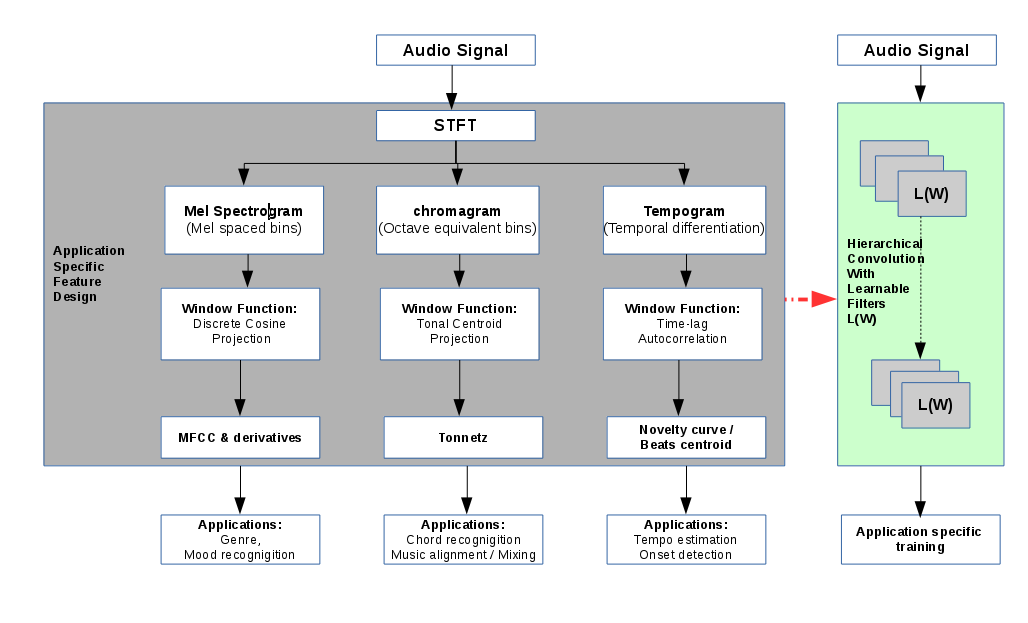
\includegraphics[width=0.95\textwidth]{dnn_motivation}
\caption{General purpose feature extractor}
 \label{fig:deep learning}
 \end{figure}
\FloatBarrier
\bigskip

\section{Temporal Approximation}
\label{temporal}
The dimension of features computed through reduction operations discussed in the previous section depends on length of the audio. But classifiers like \textit{support vector machines} and \textit{multi layer perceptron} requires features of fixed size. Therefore, frame-wise features over time are approximated to a fixed size feature representation. Temporal approximation $T$ of the reduced representation $\textbf{Y}$ is  
\[
\textbf{f} = T(\textbf{Y}) \qquad \textbf{f} \in \mathbb{R}^{Z}, \textbf{Y} \in \mathbb{R}^{T \times W}
\]
$W$ depends on length of the audio. $\textbf{f}$ is usually the final fixed size feature that is given as input to the classifier.  
\bigskip

\noindent The transformation by approximation function $T$ is done by using one of the methods,
\begin{itemize}
\setlength\itemsep{0em}
\item \textit{unsupervised} methods involving \textit{clustering techniques} (Bag Of Frames, Gaussian mixture models)
\item \textit{supervised} methods with \textit{recurrent neural network}. 
\end{itemize} 
 
\subsection{Bag Of Frames}
\label{clustering}
In Bag of Frames(BoF) model\cite{BoF}, each reduced frame is assigned to nearest of the $Z$ cluster centers. The number of assignments made to each cluster now becomes the feature $\textbf{f}$. Number of clusters $Z$ is size of the resulting feature.
\begin{algorithm}
  \caption{$\textbf{f}$ = BagOfFrames($\textbf{Y}$) }\label{bof}
  \begin{algorithmic}[1]
    \Statex \textbf{Input :} $\textbf{Y} \in \mathbb{R}^{T \times W}$
    \Statex \textbf{Output :} $\textbf{f} \in \mathbb{R}^{Z}$
    \State $\textbf{f} = 0$
    \For{$ i \in \{0,1,..,W-1\}$}
    \State $j = \argmin\limits_{j} \norm{\textbf{Y}[:,i] - \bm{\mu}_{j}}^{2}$ \Comment{$\bm{\mu}_{j} \in \mathbb{R}^{T}, j \in \{0,1..Z-1\}$}
    \State $\textbf{f}[j] \leftarrow \textbf{f}[j] + 1$
    \EndFor
  \end{algorithmic}
\end{algorithm}
\FloatBarrier
\noindent The cluster centres are computed by clustering algorithms likes gaussian mixture models or K-Means clustering. Computation of $\bm{\mu}_{j}$ by K-Means is illustrated in algorithm \ref{alg:kmeans}. The cluster centres are computed for the entire dataset. Each of the $N$ sample track could have $W$ frame-wise features. To compute these centres, $\bm{\mu}_{j}$ are first randomly initialized. Then each frame level feature is assigned to the nearest centre. After the assignment of all frame features, the cluster centres $\bm{\mu}_{j}$ are re-computed. The frame features are then re-assigned to these new centres. This re-assignment and re-computation of $\bm{\mu}_{j}$ is iterated until convergence.  
\begin{algorithm}
  \caption{K-MEANS($\textbf{Y}_{0}, \textbf{Y}_{2},..., \textbf{Y}_{N-1}$) }\label{alg:kmeans}
  \begin{algorithmic}[1]
    \Statex \textbf{Input :} $\textbf{Y}_{n} \in \mathbb{R}^{T \times W}, n \in \{0,1,...,N-1\}$
    \Statex \textbf{Output :} $\bm{\mu}_{j} \in \mathbb{R}^{T}, j \in \{0,1,..,Z-1\}$
    \State Randomly initialize $\bm{\mu}_{j}$
    \While{$\bm{\mu}_{j}$ have not converged}
    \For{$n \in \{0,1,..,N-1\}$}
      \For{$ i \in \{0,1,..,W-1\}$}
         \State $j = \argmin\limits_{j} \norm{\textbf{Y}_{n}[:,i] - \bm{\mu}_{j}}^{2}$
          \State Assign $\textbf{Y}_{n}[:,i]$ to cluster $j$
      \EndFor
    \EndFor
   \State Recompute cluster means $\bm{\mu}_{j}$
   \EndWhile
  \end{algorithmic}
\end{algorithm}
\FloatBarrier

\subsection{Recurrent Neural Networks}
\label{rnn}
The idea behind RNN is to learn a feature representation by sequentially combining the input into an internal state $\textbf{h}$. The resulting feature ($\textbf{f}$) is a projection from this internal state.
\[ 
\textbf{f} = \textbf{W}\textbf{h}_{W} \qquad \textbf{W} \in \mathbb{R}^{Z \times K}, \textbf{h}_{W} \in \mathbb{R}^{K}
\]
\[
\textbf{h}_{W} = \bm{\Theta}(\textbf{Y}[:,W], \textbf{h}_{W-1}) \qquad \textbf{Y} \in \mathbb{R}^{T \times W}
\]
$\textbf{h}_{W}$ is the internal state after combining $W$ columns of $\textbf{Y}$. $\bm{\Theta}$ is the internal state function which sequentially combines the input. The operator $\textbf{W}$ and other operators resulting from the function $\bm{\Theta}$ are solved for optimality using a labelled dataset. These operators can be computed by training an RNN (see Section \ref{training}). The function $\bm{\Theta}$ should sufficiently hold the information from beginning to end of the sequence. RNNs face challenge in remembering the information in the earlier part of the sequence. Because of this, different flavours of RNN have been developed to hold the sequence information longer and to battle the vanishing gradient problem while training neural network. Depending on how $\bm{\Theta}$ is defined, at least two RNN architectures are popular in the literature: Long-Short Term Memory (LSTM) RNN and Gated Recurrent Unit(GRU) RNN. In this thesis, only LSTMs\cite{LSTM} are considered.   

\subsubsection{Long-Short Term Memory RNN}
The LSTM internal state is contained by three gates that control the information flow. This is done by multiplying the output of each sequence $\textbf{o}_{w}$ with the corresponding cell state function $\textbf{c}_{w}$.
\[
\textbf{h}_{w} = \textbf{o}_{w} \odot \sigma_{h}(\textbf{c}_{w}) \qquad w \in \{1,2,...,W\}
\] 
$\sigma_{h}$ is hyperbolic tangent function which projects the values between -1 and 1. The output gate $\textbf{o}_{w}$ combines the $w^{th}$ vector in sequence with the previous internal state ($\textbf{h}_{w-1}$) and projects the result between 0 and 1 with sigmoid activation ($\sigma$). This indicates the contribution of current sequence $w$ to the cell state. 
\[
\textbf{o}_{w} = \sigma(\textbf{W}_{o}\textbf{Y}[:,w] + \textbf{U}_{o}\textbf{h}_{w-1})
\]
The cell state $\textbf{c}_{w}$ acts as a conveyor belt where the information can either flow unchanged or get modified with update ($\textbf{i}_{w}$) and forget functions ($\textbf{g}_{w}$).
\[
\textbf{c}_{w} = \textbf{g}_{w} \odot \textbf{c}_{w-1} + \textbf{i}_{w} \odot \sigma_{h}(\textbf{W}_{c}\textbf{Y}[:,w] + \textbf{U}_{c}\textbf{h}_{w-1})
\] 
The operators of forget gate $\textbf{W}_{g}$ and $\textbf{U}_{g}$ control the deletion of information from the\textit{ previous} sequence. The output of $g_{w}$ is between 0 (delete the information) and 1 (keep the information). 
\[
\textbf{g}_{w} = \sigma(\textbf{W}_{g}\textbf{Y}[:,w] + \textbf{U}_{g}\textbf{h}_{w-1})
\] 
The operators of update gate $\textbf{W}_{i}$ and $\textbf{U}_{i}$ control the addition of information from the \textit{current} sequence. The output of $i_{w}$ is also between 0 and 1.
\[
\textbf{i}_{w} = \sigma(\textbf{W}_{i}\textbf{Y}[:,w] + \textbf{U}_{i}\textbf{h}_{w-1})
\] 
The operators $\textbf{W}_{o}, \textbf{U}_{o}, \textbf{W}_{i}, \textbf{U}_{i}, \textbf{W}_{g}, \textbf{U}_{g}, \textbf{W}_{c}$ and $ \textbf{U}_{c}$ are solved by training the RNN.
\bigskip

\noindent To get a fixed size temporal approximation, the RNN should project all the input sequence to a single output. This architecture of RNN is called \textit{Sequence to One} RNN. 
\begin{algorithm}
  \caption{$\textbf{f}$ = $Seq2One\_LSTM$($\textbf{Y}$) }\label{alg:s2olstm}
  \begin{algorithmic}[1]
    \Statex \textbf{Input :} $\textbf{Y} \in \mathbb{R}^{T \times W}$
    \Statex \textbf{Output :} $\textbf{f} \in \mathbb{R}^{Z}$
    \State Initialize $\textbf{h}_{0}$
    \For{$ w \in \{1,2,..,W\}$}
    \State  $\textbf{h}_{w} \leftarrow \bm{\Theta}_{LSTM}(\textbf{Y}[:,w],\textbf{h}_{w-1})$
    \EndFor
    \State $\textbf{f} = \textbf{W}\textbf{h}_{W}$
  \end{algorithmic}
\end{algorithm}
\FloatBarrier

\noindent Often times, multiple layers of RNN are used. An illustration of  two layer LSTM with a \textit{sequence to sequence} LSTM in between is shown in algorithm \ref{alg:2lstm}. The input sequence is transformed in to a hidden sequence, which is then projected to a single output by the second layer. The functions in between ($\Phi_{1}, \Phi_{2}$) represents the transition operation between the layers. Several non-linear activations and transition operations have been developed to address the problems while training deep neural network (see Sec. \ref{training}). 
  
\begin{minipage}[t]{7.5cm}
  \vspace{0pt}  
\begin{algorithm}[H]
  \caption{$\textbf{f}$ = $LSTM2(\textbf{Y})$}\label{alg:2lstm}
  \begin{algorithmic}[1]
    \Statex \textbf{Input :} $\textbf{Y} \in \mathbb{R}^{T \times W}$
    \Statex \textbf{Output :} $\textbf{f} \in \mathbb{R}^{Z}$
    \Statex
    \Statex
    \Statex
    \State $\textbf{F}_{1} = \Phi_{1}(Seq2Seq\_LSTM(\textbf{Y}))$
    \State $\textbf{f} = \Phi_{2}(Seq2One\_LSTM(\textbf{F}_{1})$
  \end{algorithmic}
\end{algorithm}
\end{minipage}%
\begin{minipage}[t]{7.5cm}
  \vspace{0pt}
\begin{algorithm}[H]
  \caption{$\textbf{F}$ = $Seq2Seq\_LSTM$($\textbf{Y}$) }\label{alg:s2slstm}
  \begin{algorithmic}[1]
    \Statex \textbf{Input :} $\textbf{Y} \in \mathbb{R}^{T \times W}$
    \Statex \textbf{Output :} $\textbf{F} \in \mathbb{R}^{Z \times W}$
    \State Initialize $\textbf{h}_{0}$
    \For{$ w \in \{1,2,..,W\}$}
    \State  $\textbf{h}_{w} \leftarrow \bm{\Theta}_{LSTM}(\textbf{Y}[:,w],\textbf{h}_{w-1})$
    \State $\textbf{F}[:,w] = \textbf{W}\textbf{h}_{W}$
    \EndFor
  \end{algorithmic}
\end{algorithm}
\end{minipage}
\FloatBarrier

\section{Multi-label Classifier}
\label{classifier}
The classifier takes the feature $\textbf{f}$ as input and performs the classification task. A \textit{discriminative} \footnote{The classification model can either be \textit{generative} (approximates class distribution) or \textit{discriminative} (approximates class boundaries). For a binary classifier, the classes are either 0 or 1} binary classifier can be formalised as, 
\[
\ell_{i} = b(\zeta_{i}) =
\begin{cases}
1, & \text{if  } \zeta_{i} > \epsilon \\
0, & \text{otherwise}
\end{cases}
\qquad i \in \{1,2,..,L\}, \ell_{i} \in \{0,1\}, \textbf{f} \in \mathbb{R}^{Z}
\]
where $b$ is a binary classifier, given the feature vector $\textbf{f}$. The output of a binary classifier $\ell_{i}$ is either 0 or 1. There are $L$ binary classifier outputs for $L$ labels. $\zeta_{i}$ is the $i^{th}$ output of the classification function $C$ and the classifier output $\ell_{i}$ is 1 if $\zeta_{i}$ is greater than certain threshold $\epsilon$ 
\[
\bm{\zeta} = C(\textbf{f}) \qquad \bm{\zeta} \in \mathbb{R}^{L}
\]
The final prediction ($\textbf{pred}$) is an index set of all classifier outputs that is equal to 1 
\[
\textbf{pred} = \{\ell_{i} | \ell_{i} = 1 \}
\]
The following equivalent notation will be used in algorithms of upcoming chapters 
\[
\textbf{pred}_{(\epsilon)} = \{ b(\zeta_{i}) | b(\zeta_{i}) = 1 \} \qquad i \in \{1,2,..,L\}
\]
The classification function $C$ projects the feature $\textbf{f}$ to the vector $\bm{\zeta}$ in the label space. Depending on how this function is defined, there are several discriminative classifiers like \textit{multi-layer perceptrons}, \textit{support vector machines}, \textit{random-forest}. In this thesis, only \textit{multi-layer perceptron} is considered.


\subsection{Two-layer perceptron}
A two layer perceptron first projects the features $\textbf{f}$ to a hidden layer $\textbf{h}$ and some element-wise non-linear operation $\Phi$ is applied.
\[
\textbf{h} = \Phi(\textbf{W}_{L1}\textbf{f}) \qquad \textbf{h} \in \mathbb{R}^{L1}, \textbf{W}_{L1} \in \mathbb{R}^{L1 \times Z}
\]
Without the non-linear operation $\Phi$, the operators $\textbf{W}_{L1}$ and $\textbf{W}$ can multiply out to generalize a single layer perceptron. The motivation for using a two layer perceptron is because single layer perceptron can approximate only linear class boundries. But \textit{universal approximation theorem}\cite{upt} states that a single hidden layer with some non-linear activation function can approximate any function. The choice of $\Phi$ will be explained in section \ref{training}. The second operator $\textbf{W}$ performs the projection from hidden vector $\textbf{h}$  
\[
\bm{\zeta} = \sigma (\textbf{W}\textbf{h}) \qquad \bm{\zeta} \in \mathbb{R}^{L}, \textbf{W} \in \mathbb{R}^{L \times L1}
\]
where $\sigma$ is a sigmoid function, which projects the output of second layer between 0 and 1. 
\begin{equation}
\label{sigmoid}
\sigma (x) = \frac{1}{1 + e^{-x}}
\end{equation}
Thus $0 \leq \zeta_{i} \leq 1$ and threshold $\epsilon$ can be set in-between 0 and 1 and eventually the final prediction $\textbf{pred}$ can be computed. 

\section{Training}
\label{training}
The iterative steps involving the computation of the operators that is optimal for our context of classification task is called \textit{training}. When we train only the operators of classifying function $C$ (that is, $\textbf{W}$ and $\textbf{W}_{L1}$), the classification performance will only be as good as the information encoded in the feature $\textbf{f}$. Let us assume that the features $\textbf{f}$ obtained as a result of transformations $R$, $D$, and $T$ is optimal for the task at hand. Hence, only the classifier $C$ is trained. The abstract prediction model is shown in algorithm \ref{abstraction}.
\begin{algorithm}
  \caption{$\textbf{pred}$ = $Model$($\textbf{a}$) }\label{abstraction}
  \begin{algorithmic}[1]
    \Statex \textbf{Input :} $\textbf{a} \in \mathbb{R}^{N}$
    \Statex \textbf{Output :} $\textbf{pred}$ \Comment{indices of predicted labels}
    \State $\textbf{X} = R(\textbf{a})$ \Comment{$\textbf{X} \in \mathbb{R}^{R \times P}$}
    \State $\textbf{Y} = D(\textbf{X})$ \Comment{$\textbf{Y} \in \mathbb{R}^{T \times W}$}
    \State $\textbf{f} = T(\textbf{Y})$ \Comment{$\textbf{f} \in \mathbb{R}^{Z}$}
    \State $\bm{\zeta} = C(\textbf{f} \quad |\textbf{W},\textbf{W}_{L1})$ \Comment{$\bm{\zeta} \in \mathbb{R}^{L}$}
    \State $\textbf{pred} = \{ b(\zeta_{i}) | b(\zeta_{i}) = 1 \}$ \Comment{$ i \in \{1,2,..,L\}, b( \zeta_{i}) \in \{0,1\}$}
  \end{algorithmic}
\end{algorithm}
\FloatBarrier
\noindent Considering a two layer perceptron for classification, $\bm{\zeta}$ is computed as,
\begin{equation}
\label{eq:mlp}
\bm{\zeta} = \sigma ( \textbf{W} \Phi (\textbf{W}_{L1}\textbf{f}))
\end{equation}
\noindent Computing $\textbf{W}$ and $\textbf{W}_{L1}$ is an inverse problem. That is, we need a target $\textbf{t}$ that approximates $\bm{\zeta}$ for true classifications from a set of observations. To do this, recall that $\bm{\zeta}$ is a $L$ dimensional vector and $L$ is the number of labels in consideration. $\zeta_{i}$ is the classifier output for $i^{th}$ label and $i \in \{1,2,..,L\}$. With sigmoid ($\sigma$) projection we know that $0 \leq \zeta_{i} \leq 1$. If we assume $t_{i}$ equal to 1 for true classifications and 0 for the rest, then the transformation operators ($\textbf{W}$ and $\textbf{W}_{L1}$) can be solved such that the classifier output $\zeta_{i}$ is close to 1 for true classifications.

\subsection{First-order gradient descent}
Solving for the operators by \textit{first-order gradient descent} involves the following steps : 
\begin{enumerate}
\setlength\itemsep{0em}
\item Initialize $\textbf{W}, \textbf{W}_{L1}$
\item Run the model for a sample and compute loss $E$ = $loss(\bm{\zeta}, \textbf{t})$
\item Compute the gradient of loss with respect to the operators ($ \frac{\partial E}{\partial \textbf{W}}, \frac{\partial E}{\partial \textbf{W}_{L1}}$)
\item Update $\textbf{W}$ and $\textbf{W}_{L1}$
\item Recompute loss, gradients and update the parameters until convergence.
\end{enumerate}

\subsubsection{Loss function}
To train a classifier, a loss function (or error function) have to be defined. The \textit{least square} error function is sensitive to outliers in the training data. Hence \textit{cross-entropy}\cite{ml} loss function is considered. Error function defined as the negative log-likelihood is the \textit{cross-entropy} error function. \textit{Likelihood} that the parameters ($\textbf{W}, \textbf{W}_{L1}$) approximate a set of targets for label $i$ for $N$ training samples $({t_{i}}^{1}, {t_{i}}^{2},...,{t_{i}}^{N})$ is
\[
\mathcal{L} (\textbf{W}, \textbf{W}_{L1} | {t_{i}}^{1}, {t_{i}}^{2},...,{t_{i}}^{N} ) =  \displaystyle\prod_{n=1}^{N} {\zeta_{i(n)}}^{{t_{i}}^{(n)}}{(1-\zeta_{i(n)})}^{1 - {t_{i}}^{(n)}} \qquad t_{i} \in \{0,1\}
\]
where the \textit{likelihood} is 1, as the classifier output $\zeta_{i}$ approaches the target $t_{i}$. The log-likelihood is taken to get rid of the multiplication that would cause numerical problems over large $N$. The negative of the log-likelihood is taken to pose the optimization as a \textit{minimization} problem. Therefore, minimizing the \textit{cross-entropy} loss for label $i$ is equivalent to minimizing the \textit{negative log likelihood}
\[
\text{Minimize } E_{i}  = -ln(\mathcal{L}) = - \displaystyle\sum_{n=1}^{N} \{ {t_{i}}^{(n)} ln \zeta_{i(n)} + (1-{t_{i}}^{(n)}) ln (1-\zeta_{i(n)}) \}
\]
For $L$ labels, the total loss is minimized,
\[
\text{Minimize } \displaystyle\sum_{i=1}^{L}E_{i} 
\]
Moreover, with gradient descent optimization, the loss is minimized for a batch of samples ($B$) for every iteration. $B$ is called the \textit{batch-size}. Thus, loss for every iteration would be,
\[
{E_{i}}^{(B)} = - \displaystyle\sum_{i=1}^{L}\displaystyle\sum_{n=1}^{B} \{ {t_{i}}^{(n)} ln \zeta_{i(n)} + (1-{t_{i}}^{(n)}) ln (1-\zeta_{i(n)}) \}
\]

\subsubsection{Computing gradients}
After every iteration, the gradient of the total loss ($E$) with respect to the parameters ($\textbf{W}, \textbf{W}_{L1}$) have to computed. This gradient will then be used to update the parameters for next iteration. The gradients are computed by applying the chain rule. An illustration for computing the gradients for the two layer perceptron is shown
\begin{equation}
\label{grad1}
\frac{\partial E}{\partial \textbf{W}} = \frac{\partial E}{\partial \bm{\zeta}}  \frac{\partial \bm{\zeta}}{\partial \sigma}  \frac{\partial \sigma}{\partial \textbf{W}}
\end{equation}
\begin{equation}
\label{grad2}
\frac{\partial E}{\partial \textbf{W}_{L1}} = \frac{\partial E}{\partial \bm{\zeta}}  \frac{\partial \bm{\zeta}}{\partial \sigma}  \frac{\partial \sigma}{\partial \Phi} \frac{\partial \Phi}{\partial \textbf{W}_{L1}}
\end{equation}
Efficient computation of the gradients is achieved with \textit{back-propagation} algorithm. To ease the computations, the non-linearities and loss functions are usually chosen in such a way that the variables required for gradient computation are known in the forward pass.

\subsubsection{Updating the parameters}
Standard stochastic gradient descent update for every iteration is,
\[
\textbf{W} = \textbf{W} - \eta \frac{\partial E}{\partial \textbf{W}}
\]
where $\eta$ is the learning rate. But choosing a proper learning rate is difficult because if $\eta$ is too small, convergence can be too slow, while $\eta$ that is too high can hinder convergence. Additionally, the same learning rate is applied to all parameters across the layers. Moreover, the neural networks lead to highly non convex optimization problem and to avoid getting trapped in a local optima is challenging. Therefore, several optimization algorithms specialized for neural network training emerged to deal with the aforementioned challenges. In this thesis, Adaptive Moment (ADAM) Estimation updates\cite{adam} will be used. ADAM uses the exponentially decaying average of past moments (first moment $m$ and second moment $v$) and squared gradients ($g$) to update the parameters. Update for iteration $t$ is,
\[
m_{t} = \beta_{1}m_{t-1} + (1- \beta_{1})g_{t}
\]
\[
v_{t} = \beta_{2}v_{t-1} + (1-\beta_{2}){g_{t}}^{2}
\]
As $m_{t}$ and $v_{t}$ are initialized as vectors of 0's, the authors of ADAM observe that they are biased towards zero, especially during the initial time steps, and especially when the decay rates are small (i.e. $\beta_{1}$ and $\beta_{2}$ are close to 1). They counteract these biases by computing bias-corrected first and second moment estimates\cite{adam_o}:
\[
{m}_{t} = \frac{m_{t}}{1-{\beta_{1}}^{t}}
\]
\[
{v}_{t} = \frac{v_{t}}{1-{\beta_{2}}^{t}}
\]
Thus, update of each parameter for the next iteration is,
\[
W_{t+1} = W_{t} - \frac{\eta}{\sqrt{v_{t}} + \epsilon}m_{t}
\]
The authors propose default hyper-parameter values of 0.9 for $\beta_{1}$, 0.999 for $\beta_{2}$, and ${10}^{-8}$ for $\epsilon$

\subsection{Deep learning}
As mentioned before, if we train only the operators of classifying function $C$, then the classification performance will only be as good as the information encoded in the feature $\textbf{f}$. But, if it is possible to solve for the transformation operators that compute the features $\textbf{f}$, then it is possible to obtain features optimal for the considered task. That is, if we push the supervision into the temporal approximator function $T$ with a \textit{sequence to one} LSTM, then the classifier performance is no longer limited by the encodings in the feature $\textbf{f}$. Because, now the operators of RNN can be solved for optimality in addition to the operators of 2 layer perceptron, and therefore $\textbf{f}$ can be optimal for the task. Now we have to update every iteration not just $\textbf{W}, \textbf{W}_{L1}$, but also $\textbf{W}_{o}, \textbf{U}_{o}, \textbf{W}_{i}, \textbf{U}_{i}, \textbf{W}_{g}, \textbf{U}_{g}, \textbf{W}_{c}$ and $ \textbf{U}_{c}$   

\begin{algorithm}
  \caption{$\textbf{pred}$ = $Model$($\textbf{a}$) }\label{abstraction2}
  \begin{algorithmic}[1]
    \Statex \textbf{Input :} $\textbf{a} \in \mathbb{R}^{N}$
    \Statex \textbf{Output :} $\textbf{pred}$ \Comment{indices of predicted labels}
    \State $\textbf{X} = R(\textbf{a})$ \Comment{$\textbf{X} \in \mathbb{R}^{R \times P}$}
    \State $\textbf{Y} = D(\textbf{X})$ \Comment{$\textbf{Y} \in \mathbb{R}^{T \times W}$}
    \State $\textbf{f} = Seq2One\_LSTM(\textbf{Y} \quad | \textbf{W}_{k}, \textbf{U}_{k})$ \Comment{$ k = \{ i_{r},o,g,c\}, \textbf{f} \in \mathbb{R}^{Z}$}
    \State $\bm{\zeta} = C(\textbf{f} \quad |\textbf{W},\textbf{W}_{L1})$ \Comment{$\bm{\zeta} \in \mathbb{R}^{L}$}
    \State $\textbf{pred} = \{ b(\zeta_{i}) | b(\zeta_{i}) = 1 \}$ \Comment{$ i \in \{1,2,..,L\}, b( \zeta_{i}) \in \{0,1\}$}
  \end{algorithmic}
\end{algorithm}
\FloatBarrier
\noindent However, the performance is still limited by the frame-wise features $\textbf{Y}$. But the supervision can be further pushed inside by using convolution neural networks and solving for it's operators ($\textbf{W}_{C1}, \textbf{W}_{C2}, \textbf{W}_{C3}$) in addition to the operators of RNN and perceptron.
\begin{algorithm}
  \caption{$\textbf{pred}$ = $Model$($\textbf{a}$) }\label{abstraction3}
  \begin{algorithmic}[1]
    \Statex \textbf{Input :} $\textbf{a} \in \mathbb{R}^{N}$
    \Statex \textbf{Output :} $\textbf{pred}$ \Comment{indices of predicted labels}
    \State $\textbf{X} = R(\textbf{a})$ \Comment{$\textbf{X} \in \mathbb{R}^{R \times P}$}
    \State $\textbf{Y} = CNN(\textbf{X} \quad | \textbf{W}_{C1}, \textbf{W}_{C2}, \textbf{W}_{C3})$ \Comment{$\textbf{Y} \in \mathbb{R}^{T \times W}$}
    \State $\textbf{f} = Seq2One\_LSTM(\textbf{Y} \quad | \textbf{W}_{k}, \textbf{U}_{k})$ \Comment{$ k = \{ i_{r},o,g,c\}, \textbf{f} \in \mathbb{R}^{Z}$}
    \State $\bm{\zeta} = C(\textbf{f} \quad |\textbf{W},\textbf{W}_{L1})$ \Comment{$\bm{\zeta} \in \mathbb{R}^{L}$}
    \State $\textbf{pred} = \{ b(\zeta_{i}) | b(\zeta_{i}) = 1 \}$ \Comment{$ i \in \{1,2,..,L\}, b( \zeta_{i}) \in \{0,1\}$}
  \end{algorithmic}
\end{algorithm}
\FloatBarrier
\noindent From the illustration in algorithm \ref{MFCC_learn}, it can be seen that the learning problem can pushed up to the point of even replacing the $STFT$ operators. That is, the model can be now trained to detect the pattern directly from the raw audio signal for our classification task. Since the training data is now able to affect the operators of feature computations, the context of learning problem is now called \textit{deep learning} 

\subsubsection{Issues}
\label{issues}
As exciting as it may sound, deep learning has two major issues,\\
\\
\textit{\textbf{Requires large training data} :}\\
\\
Looking at all the application domains where deep learning is successful (image /speech recognition), they are the ones where acquiring a lot of data is feasible. As the number of parameters to optimize increases, not only that more iterations are needed to converge, but there is also a risk that the solutions converge to learning the noise in data. This is called \textit{over-fitting}.\\
\\
\textit{Transfer-learning :} This is one way to address this issue for smaller datasets. \textit{Transfer learning} is possible only when an alternate large dataset for similar task (\textit{source task}) is available. It is  then possible to train with the smaller dataset by initializing the weights with the values converged in the source task. This is called \textit{fine-tuning} the model.\\
\\
\textit{Drop-out :} This is a regularizer that counter over fitting by randomly setting parameters to zero. This is called \textit{dropping} the connection. At each training iteration, the connections can be \textit{dropped out} with probability $p$. ($Drop_{(p)}$)\\  
\\
\textit{\textbf{Vanishing gradients} :}\\  
\\
As the number of layers in the neural network increases, the risk of gradients approaching zero in the earlier layers increases. This will increase the number of iterations required for convergence. As an illustration, looking at the gradient computation equations for the final layer in equation \ref{grad1} and the penultimate layer in equation \ref{grad2}, it can be seen that as we move deeper, the number of multiplications in the chain rule required for calculating the gradient increases. If one of those gradients in chain have a value close to zero, then the gradient with respect to the parameters will also be close to zero. Thus, the non-linearities $\Phi$ are chosen such that the gradient is boosted. The non-linearities - Rectified linear units ($ReLU$)\cite{relu} and Exponential linear units ($ELU$)\cite{elu} have been used in this thesis.  
\[
ReLU(x) = max(0,x)
\]     
\[
ELU(x) = 
\begin{cases}
x, & \text{if } x \geq 0 \\
a(e^{x}-1), & \text{otherwise}
\end{cases}
\]
where $a > 0$ is a hyper-parameter.